\chapter{Fuentes Reguladas de Tensión}


\section{Introducción}

{\hspace{10pt}} Para convertir la corriente alterna de la red en corriente continua
se utilizan circuitos rectificadores. Un ejemplo de este tipo de
circuitos es el rectificador de onda completa con filtro a capacitor
mostrado en la figura \ref{fuentes1}, en dicha figura se ve
también la tensión de salida $V_S$ en función del tiempo. Esta
tensión a la salida puede no ser lo suficientemente "continua",
presentando un rizado y variaciones debido a la carga, a la
temperatura, etc.

Si el circuito electrónico que va a ser alimentado por esta fuente
necesita una tensión más estabilizada y constante frente a estas
variaciones, será necesario diseñar un circuito de estabilización o
regulación para conseguir dicho objetivo.

En forma general las posibles razones por las que el circuito de la
figura \ref{fuentes1} puede no cumplir en forma adecuada con las
necesidades en ciertas aplicaciones que requieran de tensiones
estables son:
\begin{itemize}
	\item La tensión de la red puede tener variaciones importantes.
	\item El circuito de carga (simulado por $R_L$) puede absorber
	más o menos corriente, por lo que las caídas de tensión en el
	transformador y en los diodos producirán variaciones apreciables
	en el valor medio de la tensión de salida.
	\item El circuito rectificador deja pasar componentes alternas
	de rizado.
	\item El valor medio de la tensión de salida varía con la
	temperatura debido a la utilización de semiconductores.
\end{itemize}

Por lo tanto si se requiere precisión en la tensión de alimentación,
es necesario un circuito estabilizador o regulador. Intentando
reducir, dentro de lo posible, los efectos antes mencionados.


\begin{figure}
	\centering
	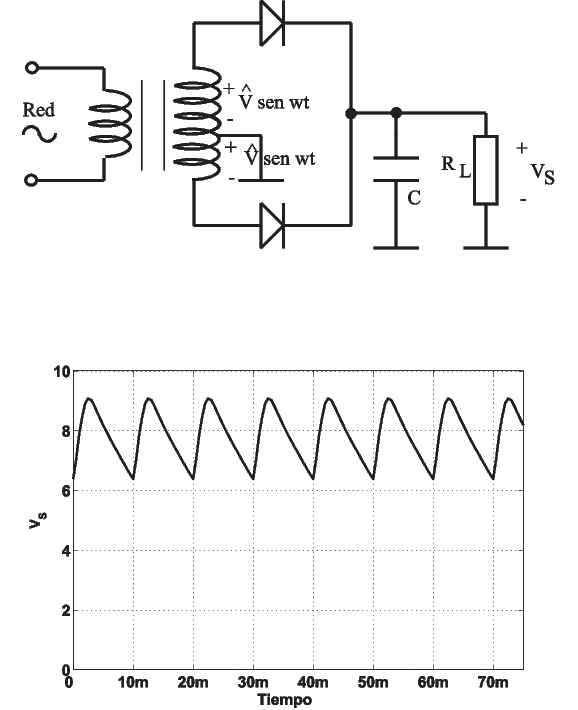
\includegraphics[width=3.5in]{figuras/fuente1x.png}\\
	\caption{Rectificador de onda completa. Tensión de salida $V_S$ en función del tiempo}\label{fuentes1}
\end{figure}

\section{Parámetros característicos de una fuente regulada}


{\hspace{10pt}} El sistema mostrado en la figura \ref{fuentes2} es una fuente de
tensión regulada, si teniendo en cuenta las posibles perturbaciones:

\begin{equation}
	\frac{\displaystyle \triangle V_S}{\displaystyle V_S}<
	\frac{\displaystyle \triangle V_e}{\displaystyle V_e}
\end{equation}


\begin{figure}
	\centering
	
\includegraphics[width=3in]{figuras/fuentes2.png}\\
	\caption{Fuente regulada de tensión. Perturbaciones más apreciables}\label{fuentes2}
\end{figure}

Para evaluar la calidad y características de funcionamiento de una
fuente se definen los siguientes parámetros:

\medskip

\textbf{Factor de regulación.}

\medskip

Se define como factor de regulación $F_R$, la siguiente expresión:

\begin{equation}
	F_R=\frac{\displaystyle \triangle V_S}{\displaystyle \triangle
		V_e}\biggr |_{\triangle T=0, \quad \triangle I_S=0}
\end{equation}

Este factor da una idea de la variación de la salida en función de
la variación en la entrada y deberá ser lo menor posible.

Cuando lo que se analiza es la variación de la salida debido a la
variación del valor medio de la tensión de entrada $V_e$, se
utilizan modelos de gran señal y se denomina factor de regulación de
línea. Cuando lo que se analiza es el rizado en la salida debido al
rizado en la entrada, se utilizan modelos de pequeña señal y el
factor se denomina factor de regulación del ripple.

Se utiliza también este factor en su forma relativa y porcentual:

\begin{equation}
	F'_R\%=\frac{\displaystyle \frac{\triangle V_S}{V_S}}{\displaystyle \triangle
		\frac{V_e}{V_e}}100\%
\end{equation}

Para tener una referencia práctica fuentes de gran calidad deberán
tener un $F'_R\%<0,01\%$ y fuentes de calidad media pueden tener un
$F'_R\% \approx 0,1\%$.


\medskip

\textbf{Resistencia de salida.}

\medskip

Por definición la resistencia de salida será:

\begin{equation}
	R_S=\frac{\displaystyle \triangle V_S}{\displaystyle \triangle
		I_S}\biggr |_{\triangle V_e=0, \quad \triangle T=0}
\end{equation}

Ésta deberá ser lo más pequeña posible. La figura \ref{fuentes3}
muestra la curva de regulación de la tensión de salida en función de
la corriente de carga ($V_e=cte$). La resistencia de salida $R_S$ es
la pendiente de dicha curva, a veces se define también la
resistencia de salida total como:


\begin{equation}
	R_{S tot}=\frac{\displaystyle \triangle V_{S \quad total}}{\displaystyle I_{S \quad max}}
\end{equation}


Esta resistencia $R_S$ es la resistencia para variaciones lentas de
$I_S$, en caso de variaciones rápidas se define la impedancia de
salida $|Z_S|=\frac{\displaystyle |\triangle V_S|}{\displaystyle
	|\triangle I_S|}(w)$ que dependerá de la frecuencia.

\begin{figure}
	\centering
	
\includegraphics[width=3.5in]{figuras/fuentes3.png}\\
	\caption{Curva de regulación de carga.}\label{fuentes3}
\end{figure}

\medskip

\textbf{Coeficiente de temperatura.}

\medskip

Para estudiar la estabilidad térmica se define el coeficiente de
temperatura como:

\begin{equation}
	K_T=\frac{\displaystyle \triangle V_S}{\displaystyle \triangle
		T}\biggr |_{\triangle V_e=0, \quad \triangle I_S=0}
\end{equation}

Este parámetro debe ser lo más pequeño posible. En algunas ocasiones
se utiliza el parámetro en forma relativa ($\frac{\displaystyle
	\triangle V_S/V_S}{\displaystyle \triangle
	T}100\%$), expresándolo en tanto por ciento por grado centígrado.


\section{Teoría básica de los reguladores}

{\hspace{10pt}} La función de los reguladores de tensión es convertir una tensión de
entrada de continua, en un valor de tensión de salida de continua,
estable sobre un amplio rango de corriente de carga y ante
variaciones de las condiciones de la tensión de entrada. En la
figura \ref{fuentes4} se muestra un regulador de tensión genérico,
allí se ven los bloque básicos que son comunes a las tres
configuraciones más utilizadas (serie, paralelo y conmutación).
Dichos bloques son:

\begin{itemize}
	\item \textbf{Referencia de tensión}. Este elemento provee un
	nivel de tensión conocido y estable para utilizarlo como
	referencia.
	\item \textbf{Elemento de muestreo de tensión}. Este elemento
	toma una muestra de la tensión de salida, que comparada con la
	referencia hace que el sistema realimentado reaccione
	apropiadamente para tender a oponerse a la variación detectada
	en la salida.
	\item \textbf{Amplificador de error}. Este elemento amplifica
	las diferencias detectadas entre la tensión de referencia y la
	tensión de muestreo, para que actúe eficientemente el sistema de
	realimentación.
	\item \textbf{Elemento de control}. El elemento de control es manejado por el amplificador de
	error y su funcionamiento varía según la configuración. En la
	configuración serie se controla el pasaje de la corriente en
	serie para mantener la tensión de salida constante (ver figura \ref{fuentes5} a)), en la configuración
	paralelo se deriva corriente en paralelo (figura \ref{fuentes5}
	b)) y con la configuración conmutada se regula la apertura y
	cierre de una llave (ver figura \ref{fuentes5} c)).
\end{itemize}

\begin{figure}
	\centering
	
\includegraphics[width=3.5in]{figuras/fuentes4.png}\\
	\caption{Bloques en un regulador de tensión genérico.}\label{fuentes4}
\end{figure}

\begin{figure}
	\centering
	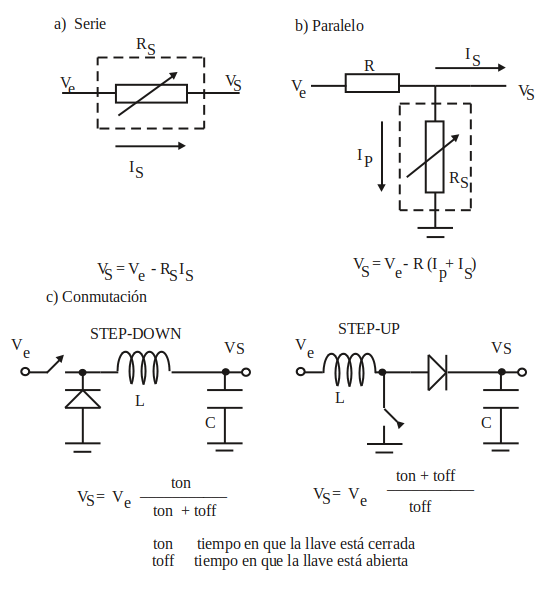
\includegraphics[width=3.5in]{figuras/fuentes5.png}\\
	\caption{Elemento de control correspondiente a: a) regulador serie, b) regulador paralelo y c) regulador de conmutación (step-down y step-up). }\label{fuentes5}
\end{figure}


\subsection{Regulador serie}

{\hspace{10pt}} En esta configuración, la tensión de salida $V_S$ es regulada
modulando la conducción de un dispositivo activo colocado en serie
con la corriente de salida. Usualmente se utiliza un TBJ que
funciona como el resistor "variable" de la figura \ref{fuentes5}
a).

En la figura \ref{fuentes6} se muestra el esquema básico de este
tipo de regulador. El divisor resistivo formado por $R_1$ y $R_2$
toma una muestra de la tensión de salida $V_S$, ésta es comparada
con la tensión de referencia $V_{REF}$; la diferencia producto de la
comparación es amplificada por el Amplificador Operacional. La
salida del AO maneja la base del TBJ y por lo tanto, si la
realimentación del sistema es negativa, las variaciones producidas
en la salida tienden a compensarse obteniéndose una regulación en la
tensión de salida. En la figura \ref{fuentes6} se asocian los
componentes del circuito con los bloques de la figura
\ref{fuentes4}, utilizando rectángulos punteados.

En la figura \ref{fuentes7} se muestra otra variante de un regulador
serie, en dónde al Amplificador de Error es implementado con un TBJ
y un generador de corriente constante.

\begin{figure}
	\centering
	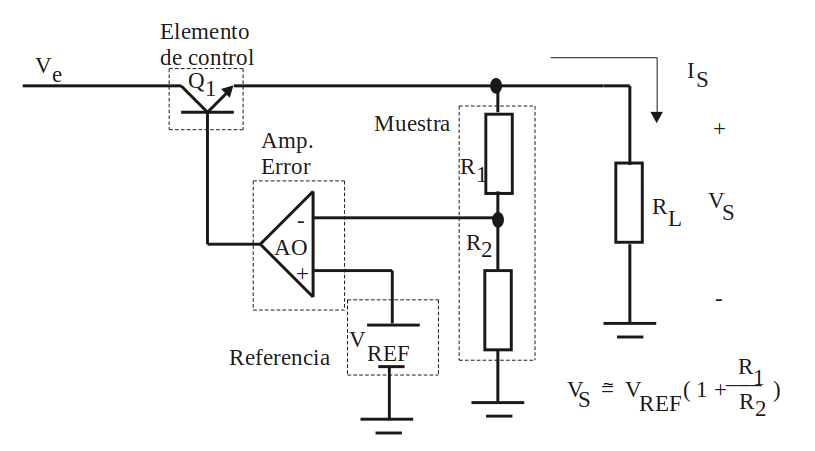
\includegraphics[width=3.5in]{figuras/fuentes6.png}\\
	\caption{Regulador serie con AO. }\label{fuentes6}
\end{figure}

\begin{figure}
	\centering
	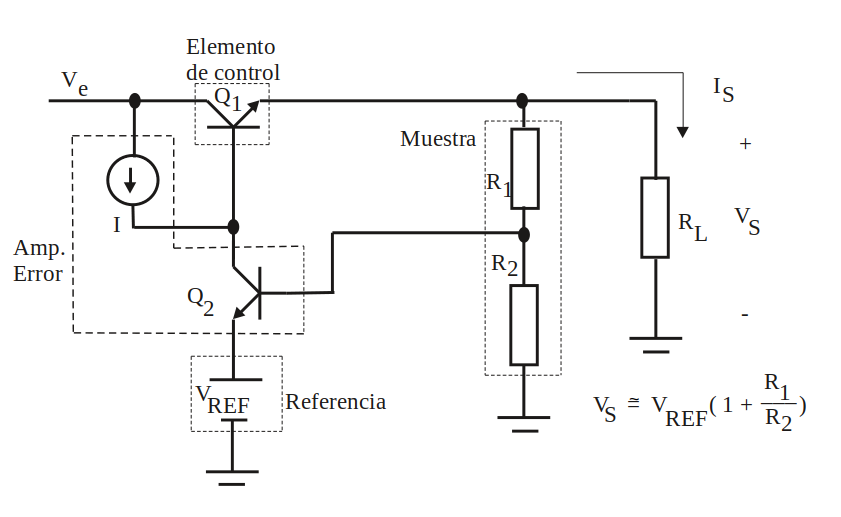
\includegraphics[width=3.5in]{figuras/fuentes7.png}\\
	\caption{Regulador serie. Amplificador de error con TBJ y generador de corriente.}\label{fuentes7}
\end{figure}

El regulador serie provee un modo sencillo  de obtener tensión
regulada. Sin embargo, si se necesita trabajar con corrientes
elevadas, el elemento de control deberá disipar una potencia elevada
debido a que toda la corriente de salida circulará a través de él,
resultando un regulador con bajo rendimiento de potencia.

\subsection{Regulador paralelo}

{\hspace{10pt}} El regulador paralelo emplea un elemento de control en paralelo en
el cual la corriente derivada por él compensa las variaciones en la
tensión de entrada o los cambios en las condiciones de carga. El
regulador paralelo básico puede verse en la figura \ref{fuentes8}.
En dicha figura el sistema realimentado mantiene la corriente
$I=I_P+I_S$ aproximadamente constante ( y por lo tanto la caída en
$R$ ) de modo que las variaciones en la corriente de carga son
absorbidas por el elemento de control.

El regulador paralelo tiene menos rendimiento que el serie y el de
conmutación. Esto se debe a que la disipación de potencia en el
elemento de control es elevada, ya que toda la tensión de salida
está aplicada sobre el dispositivo activo. Sin embargo en algunas
aplicaciones puede ser útil debido a: las variaciones en la
corriente de carga no se ven reflejadas en la fuente de entrada
($I\approx cte$), y está autoprotegido contra corto circuitos.

\begin{figure}
	\centering
	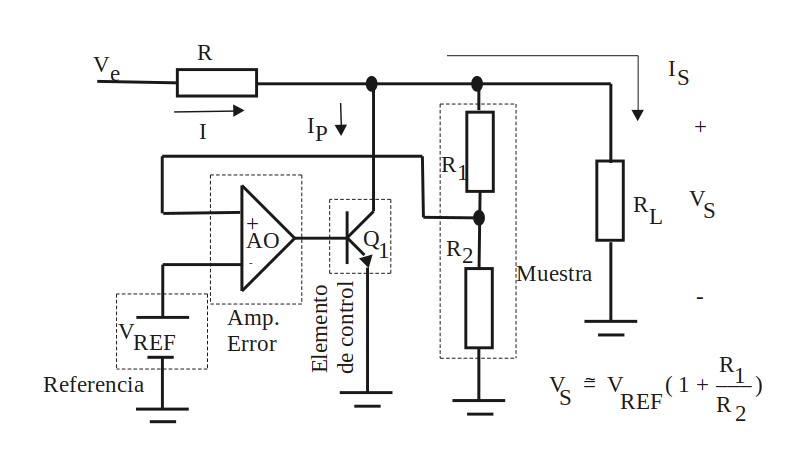
\includegraphics[width=3.5in]{figuras/fuentes8.png}\\
	\caption{Regulador paralelo.}\label{fuentes8}
\end{figure}

\subsection{Regulador de conmutación}

{\hspace{10pt}} El regulador de conmutación emplea como elemento de control una
llave activa (por ejemplo un TBJ). Esta llave se utiliza para
muestrear la tensión de entrada con un ciclo de trabajo controlado
por los requerimientos de carga. El circuito de la figura
\ref{fuentes9} es un esquema básico de un regulador de conmutación
en su variante \emph{step-down}. La tensión de entrada muestreada es
pasada a través de un filtro L-C, obteniendo a la salida una tensión
promediada para alimentar a la carga. Debido a que el TBJ que actúa
como llave está en saturación o en corte la potencia disipada en el
elemento de control es mínima, derivando esta condición en un buen
rendimiento del sistema superior a los reguladores serie y paralelo.

En el esquema presentado en la figura \ref{fuentes9} los resistores
$R_1$ y $R_2$ toman una muestra de la salida, esta muestra es
comparada con la referencia y su diferencia amplificada por el AO.
Éste maneja la modulación del ciclo de trabajo de una oscilador de
frecuencia constante.

\begin{figure}
	\centering
	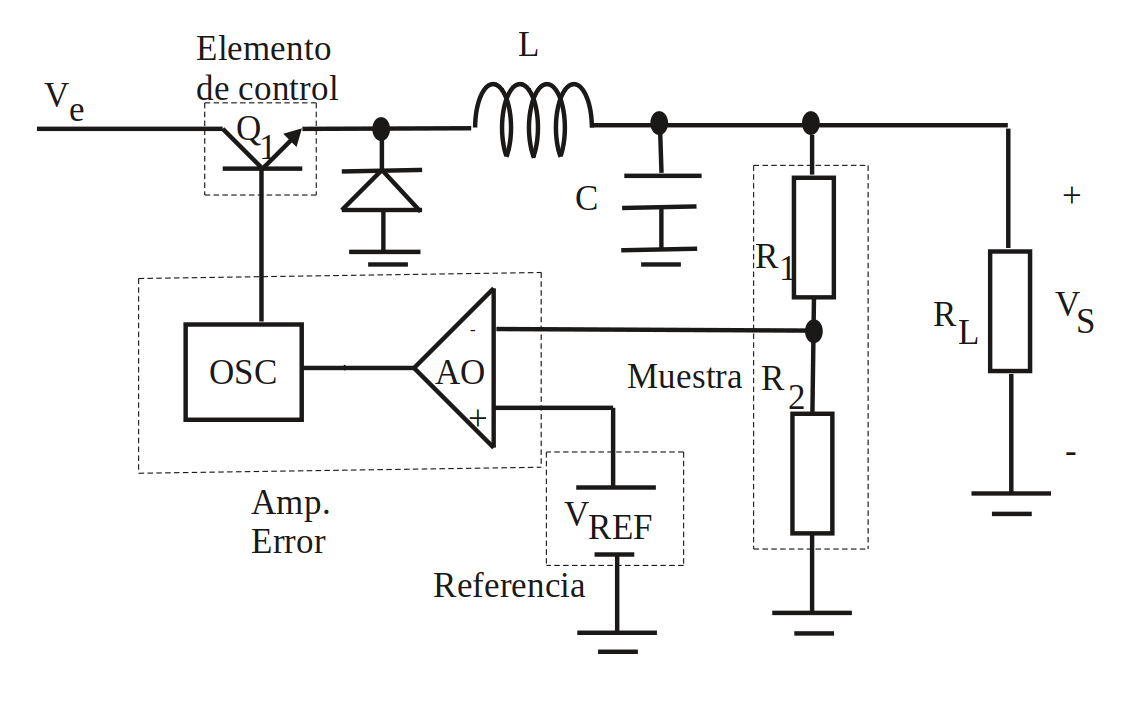
\includegraphics[width=3.5in]{figuras/fuentes9.png}\\
	\caption{Regulador de conmutación. Variante \emph{step-down}.}\label{fuentes9}
\end{figure}


\section{Ejemplo de una fuente regulada serie}

{\hspace{10pt}} La figura \ref{fuentes10} muestra un circuito elemental de una
fuente de tensión regulada serie y sigue un esquema similar al de la
figura \ref{fuentes7}.

En ella el divisor resistivo formado por $R_1$ y $R_2$ toma una
muestra de la tensión de salida, dicha muestra es comparada con la
referencia de tensión formada por el diodo Zener $DZ_1$ polarizado
con la fuente de entrada $V_i$ a través de la resistencia $R_Z$. La
diferencia entre la tensión muestreada y la referencia es
amplificada por el amplificador de error, éste está constituido por
$Q_2$, $Q_3$ y $R_E$ conectados como un amplificador diferencial. La
resistencia $R_3$ reemplaza a la fuente de corriente de la figura
\ref{fuentes7}, dándole polarización a $Q_2$ y la excursión de
corriente de base al elemento de control ($Q_1$) necesaria para
abarcar el rango de funcionamiento del regulador.


\begin{figure}
	\centering
	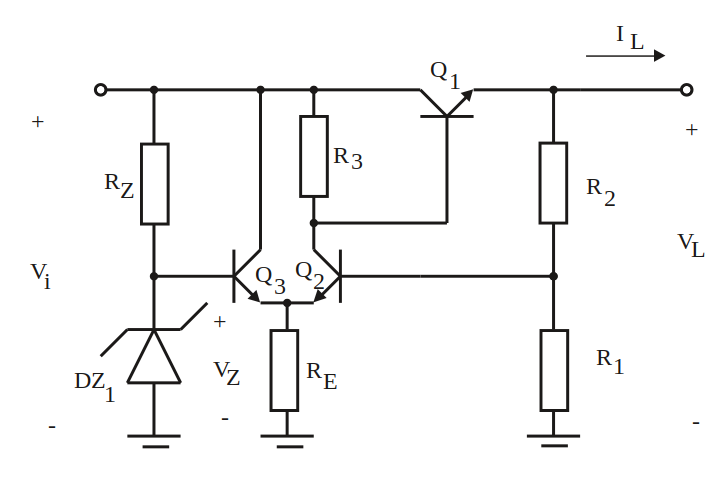
\includegraphics[width=3.5in]{figuras/fuentes10.png}\\
	\caption{Ejemplo de Regulador Serie.}\label{fuentes10}
\end{figure}


El TBJ $Q_1$ debe dimensionarse de modo que pueda disipar una
potencia dada por:

\begin{equation}
	P_{Q_1}= I_{Lmax}(V_i-V_L)\label{condicionesnormales}
\end{equation}

, en funcionamiento normal y por:

\begin{equation}\label{cortocircuito}
	P_{Q_1}= I_{Lmax}V_i
\end{equation}

, con limitación de corriente en condiciones de cortocircuito, como
se verá más adelante.

La figura \ref{fuentes11} es el detalle del elemento de control y de
la resistencia $R_3$ de la figura \ref{fuentes10}. De ella se
obtiene que:

\begin{equation}
	I_3= \frac{\displaystyle V_i-V_{BE1}-V_L}{\displaystyle
		R_3}=\frac{\displaystyle I_L}{\displaystyle \beta_1}+I_{C2}
\end{equation}

$R_3$ debe diseñarse de modo que con la máxima carga ($I_{Lmax}$),
pueda suministrar a $Q_2$ al menos una corriente $I_{C2min}$ que
asegure su funcionamiento en zona activa. De estas consideraciones
se deduce que:

\begin{equation}
	R_3\leq \frac{\displaystyle V_i-V_{BE1}-V_L}{\frac{\displaystyle I_{Lmax}}
		{\displaystyle \beta_1}+I_{C2min}}
\end{equation}

\begin{figure}
	\centering
	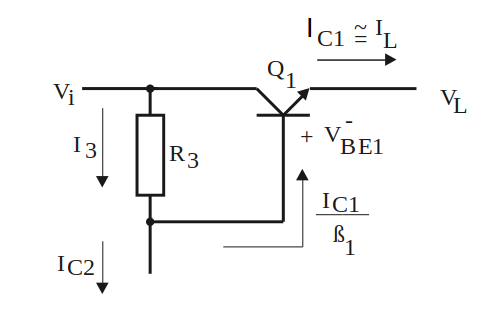
\includegraphics[width=2.5in]{figuras/fuentes11.png}\\
	\caption{Detalle del Elemento de Control.}\label{fuentes11}
\end{figure}


Cuando el regulador trabaja en vacío ($I_L=0$), la corriente
$I_{C2}$ será máxima, y podrá obtenerse de:

\begin{equation}
	I_{C2max}=\frac{\displaystyle V_i-V_{BE1}-V_L}{\displaystyle R_3}
\end{equation}

La corriente $I_E\simeq I_{C2}+I_{C3}$ que circula por la
resistencia $R_E$ hacia tierra será aproximadamente constante con
una valor:

\begin{equation}
	I_E=\frac{\displaystyle V_Z-V_{BE3}}{\displaystyle R_E}
\end{equation}

La resistencia $R_E$ y por lo tanto su corriente $I_E$ deberán
diseñarse para asegurar que en la condición de carga de vacío la
corriente $I_{C3}$, mínima en este caso, se mantenga dentro de un
valor que asegure la polarización de $Q_3$ dentro de la zona activa.
por lo tanto:

\begin{equation}
	I_E\geq I_{C2max}+I_{C3min}
\end{equation}

\begin{equation}
	R_E\leq  \frac{\displaystyle V_Z-V_{BE3}}{\displaystyle I_{C2max}+I_{C3min} }
\end{equation}


La tensión de base de $Q_2$ es aproximadamente igual a la tensión de
referencia dada por el diodo Zener. Con esta consideración, el
divisor resistivo formado por $R_1$ y $R_2$ se diseña para que la
tensión de salida sea $V_L$, suponiendo que la corriente que
atraviesa el divisor es mucho mayor que la corriente de base de
$Q2$, es decir:

\begin{equation}
	V_L\simeq V_Z \frac{\displaystyle R_1+R_2}{\displaystyle R_1}
\end{equation}

Para analizar el comportamiento del regulador frente al rizado o
"ripple" de la tensión de entrada se utiliza el modelo de pequeña
señal de los dispositivos activos. Se supone una entrada de señal
$v_i$ y se analiza la salida $v_L$.

Hay dos caminos de propagación del "ripple", uno a través de la
resistencia dinámica del Zener y otro a través de la resistencia
$R_3$. Se puede analizar el efecto de cada uno por separado
superponiendo sus resultados para obtener el factor de regulación
del ripple total.

El circuito equivalente de pequeña señal que permite analizar el
primero de estos efectos se muestra en la figura \ref{fuentes12} a).
En ella se realizó un equivalente de Thèvenin entre la resistencia
dinámica del diodo Zener $r_Z$ y su resistencia de polarización
$R_Z$. El extremo de la resistencia $R_3$ conectado a la entrada se
puso a tierra, ya que se anuló el efecto de la misma por ese camino.
Es de notar que por simplicidad se dibujó a los TBJs con su esquema
general, pero debe entenderse ese dibujo como su modelo de pequeña
señal.

De la figura \ref{fuentes12} a) se puede ver que el circuito es un
amplificador realimentado con configuración serie-paralelo (ver
capítulo 1). En él la red de realimentación está determinada por las
resistencias $R_1$ y $R_2$. En consecuencia si la ganancia de lazo
es $T\gg 1$ la ganancia de tensión será:


\begin{equation}
	\frac{\displaystyle v_L}{\displaystyle v_{TH}}\simeq \frac{\displaystyle R_1+R_2}{\displaystyle R_1}
\end{equation}

Cómo $v_{TH}=v_i\frac{\displaystyle r_Z}{\displaystyle r_Z+R_Z}$,
por lo tanto:

\begin{equation} \label{ecuacion1}
	v_L\mid_1 \simeq v_i \frac{\displaystyle R_1+R_2}{\displaystyle R_1} \frac{\displaystyle r_Z}{\displaystyle r_Z+R_Z}
\end{equation}


\begin{figure}
	\centering
	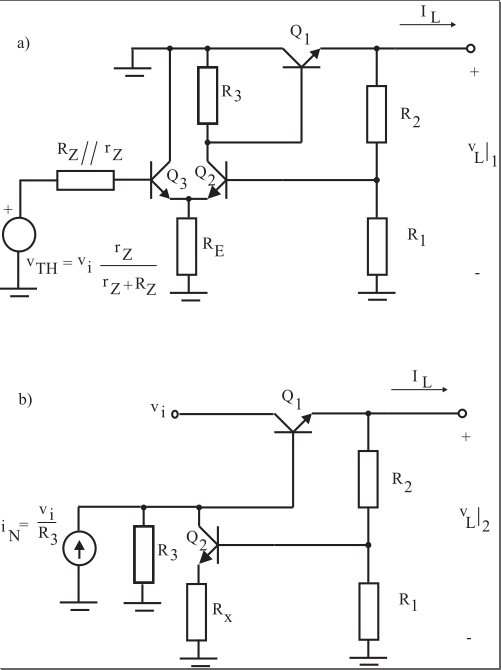
\includegraphics[width=3.5in]{figuras/fuentes12.png}\\
	\caption{Circuito de pequeña señal para analizar el ripple. a) entrando por el Zener, b) por $R_3$ .}\label{fuentes12}
\end{figure}

El segundo camino de entrada del ``ripple'' se esquematiza en la
figura \ref{fuentes12} b). En este circuito la entrada
correspondiente al Zener se pone a tierra; por lo tanto el emisor de
$Q_2$ ``ve'' una resistencia:

\begin{equation}
	R_x=R_E \parallel \frac{\displaystyle h_{ie3}+R_Z\parallel r_z }{\displaystyle h_{fe3}+1}
\end{equation}

En la entrada $v_i$ y $R_3$ se aplica el teorema de Norton y el
colector de $Q_1$ se separa del circuito, ya que la señal no ingresa
por él.

El circuito de la figura \ref{fuentes12} b) corresponde a una
configuración de realimentación paralelo-paralelo, en el cual la red
de realimentación está formada por $R_1$, $R_2$, $R_x$ y $Q_2$. El
parámetro $y_{12}$ de la red de realimentación será:


\begin{equation}\label{ecuacion1-1}
	f_y=y_{12}=h_{fe2}\quad \frac{\displaystyle 1 }{\displaystyle
		h_{ie2}+(h_{fe2}+1)R_x} \quad \frac{\displaystyle R_1\parallel (h_{ie2}+(h_{fe2}+1)R_x)
	}{\displaystyle R_1\parallel (h_{ie2}+(h_{fe2}+1)R_x)+R_2}
\end{equation}


Si la ganancia de lazo $T\gg1$, la transferencia
$A_z=\frac{\displaystyle v_L}{\displaystyle i_N}\simeq
\frac{\displaystyle 1}{\displaystyle f_y}$, como
$i_N=\frac{\displaystyle v_i}{\displaystyle R_3}$, por lo tanto:


\begin{equation} \label{ecuacion2}
	v_L\mid_2 \simeq v_i \frac{\displaystyle 1}{\displaystyle f_yR_3}
\end{equation}

De las ecuaciones \ref{ecuacion1} y \ref{ecuacion2} se puede obtener
el factor de regulación del ripple:

\begin{equation}
	F_R  = \frac{\displaystyle v_L}{\displaystyle v_i}=\frac{\displaystyle R_1+R_2}{\displaystyle R_1} \frac{\displaystyle r_Z}{\displaystyle
		r_Z+R_Z}+\frac{\displaystyle 1}{\displaystyle f_yR_3}
\end{equation}


Para el cálculo de la resistencia de salida se utiliza el circuito
de la figura \ref{fuentes13}, en este circuito se reemplazó la red
de relimentación del circuito de la figura \ref{fuentes12} b) por su
equivalente en parámetros admitancia. Siendo $y_{12}$ lo expresado
en la ecuación \ref{ecuacion1-1}, e $y_{22}$ el efecto de carga a la
salida de la red de realimentación dado por:

\begin{equation}
	y_{22}  = \frac{\displaystyle 1}{\displaystyle R_2+R_1\parallel (h_{ie2}+(h_{fe2}+1)R_x)}
\end{equation}

De la figura \ref{fuentes13} se deduce que la resistencia de salida
$R_o$ es:


\begin{equation}
	\nonumber
	v_L = i_x \frac{\displaystyle h_{ie1}}{\displaystyle h_{fe1}+1}+R_3\left(\frac{\displaystyle i_x}{\displaystyle h_{fe1}+1}-y_{12}v_L\right)
\end{equation}
\begin{equation}
	\nonumber
	\frac{\displaystyle v_L}{\displaystyle i_x}= \frac{\displaystyle \frac{\displaystyle h_{ie1}+R_3}{\displaystyle h_{fe1}+1}}{\displaystyle 1+R_3y_{12}}
\end{equation}
\begin{equation}
	R_o = \frac{\displaystyle 1}{\displaystyle y_{22}}\parallel
	\frac{\displaystyle v_L}{\displaystyle i_x}
\end{equation}


\begin{figure}
	\centering
	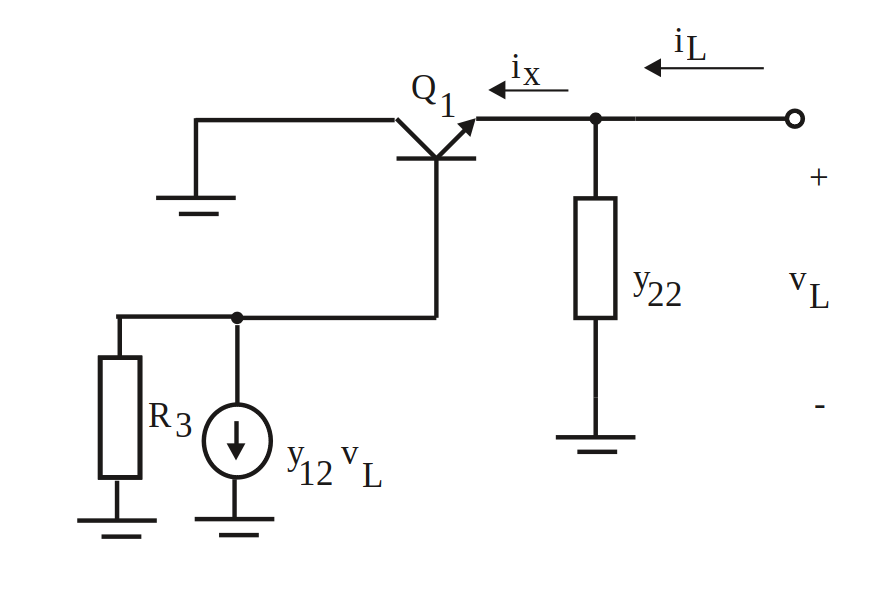
\includegraphics[width=3in]{figuras/fuentes13.png}\\
	\caption{Circuito de pequeña señal para analizar la resistencia de salida.}\label{fuentes13}
\end{figure}

\subsection{Protección contra corto circuito}

{\hspace{10pt}} El circuito de la figura \ref{fuentes14} a) es una posible
protección contra corto circuitos aplicada al circuito básico de la
figura \ref{fuentes10}. La resistencia $R_{SC}$ está en serie con la
corriente de carga $I_L$ sensándola. El transistor $Q_4$ se
encuentra al corte en condiciones normales de trabajo, ya que su
tensión $V_{BE4}$ (caída sobre $R_{SC}$) no es suficiente para
encenderlo. Cuando la corriente llega al valor máximo diseñado el
transistor $Q_4$ se enciende tomando corriente e impidiendo que la
corriente de base de $Q_1$ (y por lo tanto $I_L$) aumente
desmedidamente. El valor de diseño de $R_{SC}$ debe ser:

\begin{equation}
	R_{SC}=\frac{\displaystyle V_{BE4(on)}}{I_{Lmax}}
\end{equation}

En la figura \ref{fuentes14} b) se muestra el comportamiento
cualitativo de la tensión de salida $V_L$ en función de la corriente
de carga, del regulador protegido contra corto circuitos. La
corriente $I_{Lo}$ es levemente superior a $I_{Lmax}$ debido a la
corriente de emisor de $Q_4$.

\begin{figure}
	\centering
	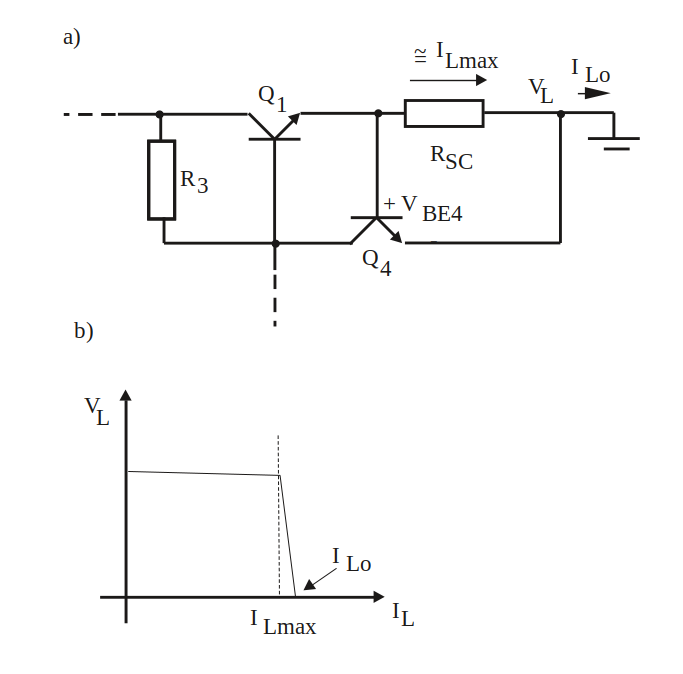
\includegraphics[width=3.5in]{figuras/fuentes14x.png}\\
	\caption{Protección contra corto circuitos. a) Circuito en condición de corto circuito, b) curva de regulación de salida.}\label{fuentes14}
\end{figure}


En condiciones de corto circuito esta protección determina que el
transistor $Q_1$ se diseñe para soportar las condiciones dadas en la
ecuación \ref{cortocircuito}, lo que puede derivar en una
sobredimensionamiento de dicho transistor con respecto a las
condiciones normales de funcionamiento (ver ecuación
\ref{condicionesnormales}).

Para mejorar esta característica se utiliza un circuito con
protección con "repliegue" (\emph{fold back}) como se muestra en
la figura \ref{fuentes15} a).

En la figura \ref{fuentes15} b) se ve el comportamiento cualitativo
de la tensión de salida $V_L$ en función de la corriente de carga,
del regulador con repliegue. Este comportamiento asegura que en
condiciones de cortocircuito la potencia que debe disipar $Q_1$
estará dada por:

\begin{equation}
	P_{Q_1} \simeq I_{FB}V_i
\end{equation}

Este repliegue de la corriente se debe a la realimentación positiva
suministrada por $Q_4$ cuando éste se enciende ($I_L=I_{Lmax}$). Las
ecuaciones de diseño son las siguientes:

\begin{equation}
	\frac{\displaystyle R_B}{\displaystyle
		R_A+R_B}(I_{Lmax}R_{SC}+V_o)-V_o=V_{BE4(on)}
\end{equation}
, en el momento previo al encendido de $Q_4$ y:
\begin{equation}
	I_{FB}\simeq \frac{\displaystyle V_{E1}}{\displaystyle R_{SC}} \simeq
	\frac{\displaystyle V_{BE4}}{\displaystyle R_{SC}} \left(\frac{\displaystyle R_B+R_A}{\displaystyle
		R_B}\right)
\end{equation}
, funcionando el repliegue y suponiendo que $I_{FB} \gg I_{E4}$ e
$I_{B4}\ll I_X$.


\begin{figure}
	\centering
	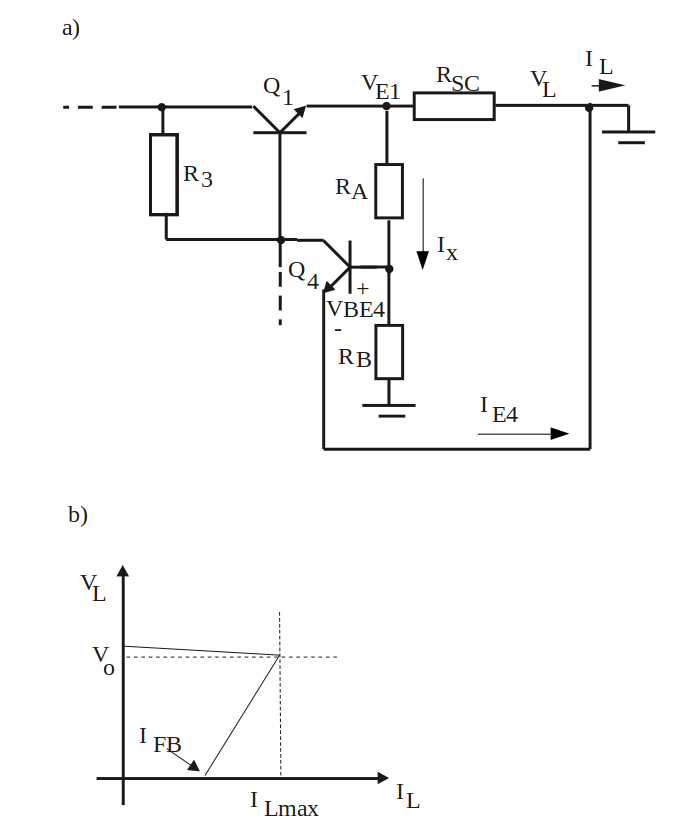
\includegraphics[width=3.5in]{figuras/fuentes15x.png}\\
	\caption{Protección con repliegue. a) Circuito en condición de corto circuito, b) curva de regulación de salida.}\label{fuentes15}
\end{figure}


\section{Fuentes reguladas serie integradas}

{\hspace{10pt}} Existen gran cantidad de circuitos integrados que cumplen con la
función de regular tensión. Los hay de tensiones fijas y ajustables,
con diversas características de manejo de corriente y de desempeño.

Para ilustrar estas posibilidades se describen dos reguladores muy
utilizados, el $\mu A723$ y el LM317.

En la figura \ref{fuentes16} se muestra el diagrama en bloques del
regulador $\mu A723$. En ella se distinguen a la izquierda el
Amplificador Operacional $A_1$, el diodo Zener y el generador de
corriente que forman la referencia de tensión con salida en el pin
$V_{REF}$. En el centro el Amplificador Operacional $A_2$ que será
el que realice la función de amplificador de error, con entradas en
los pines $V^+$ y $V^-$. Y a la derecha los transistores $Q_o$ y
$Q_1$ que serán el elemento de control serie y el encargado de
proveer protección contra corto circuitos respectivamente, en ellos
se distinguen los pines $+V_C$, $OUT$, $CURRENT \quad SENSE \quad
(CS)$, $CURRENT \quad LIMIT \quad (CL)$ y $COMPENSACION \quad (C)$.
Este circuito integrado está alimentado a través de los pines
$+V_{cc}$ y $-V_{cc}$.


\begin{figure}
	\centering
	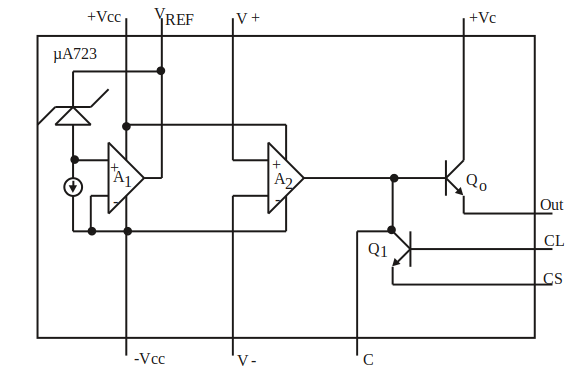
\includegraphics[width=3.5in]{figuras/fuentes16.png}\\
	\caption{Diagrama en bloques del circuito integrado $\mu A723$.}\label{fuentes16}
\end{figure}

Si se realizan las conexiones adecuadas y se agregan los componentes
necesarios se puede lograr una configuración de un regulador serie
similar a la presentada en la figura \ref{fuentes6}. Teniendo en
cuenta además que el valor típico de la tensión de referencia en
este circuito integrado es de $V_{REF}=7,15V$, se pueden diseñar
reguladores ajustables entre 2 y 7V (figura \ref{fuentes17}) y entre
7 y 37V (figura \ref{fuentes18}. Como la capacidad de corriente que
es capaz de entregar el integrado es limitada ($\simeq 50mA$), se la
puede aumentar con el agregado de transistores de potencia, como se
muestra en la figura \ref{fuentes19}.

\begin{figure}
	\centering
	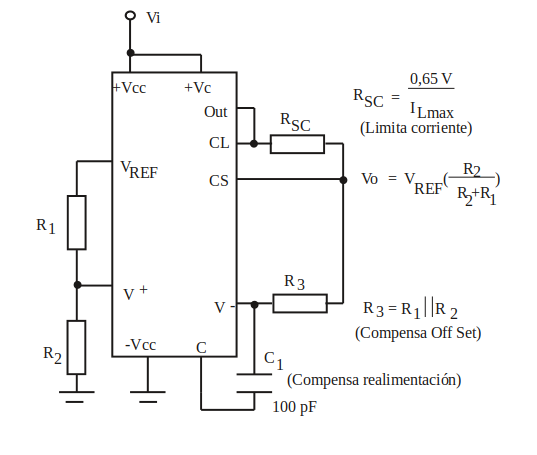
\includegraphics[width=3.5in]{figuras/fuentes17.png}\\
	\caption{Utilización del $\mu A723$ como regulador entre 2 y 7V.}\label{fuentes17}
\end{figure}

\begin{figure}
	\centering
	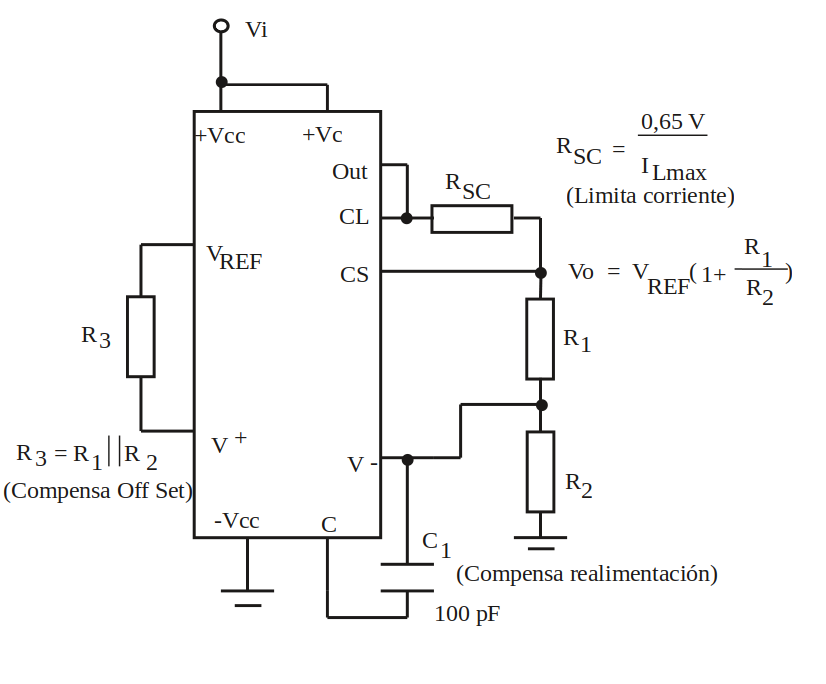
\includegraphics[width=3.5in]{figuras/fuentes18.png}\\
	\caption{Utilización del $\mu A723$ como regulador entre 7 y 37V.}\label{fuentes18}
\end{figure}

\begin{figure}
	\centering
	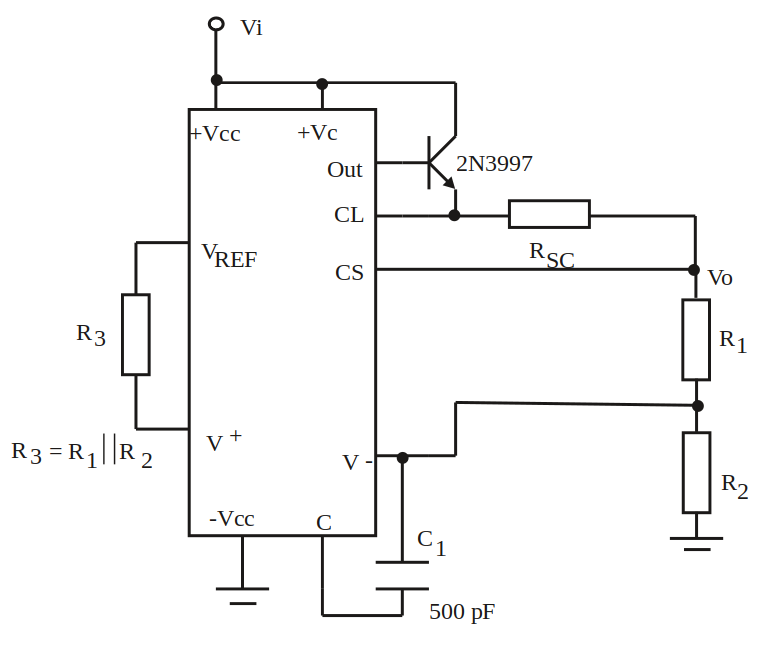
\includegraphics[width=3.5in]{figuras/fuentes19.png}\\
	\caption{Aumento de la capacidad de corriente del circuito de la figura \ref{fuentes18}.}\label{fuentes19}
\end{figure}


Otro circuito integrado muy utilizado es el LM317 de tres
terminales. En la figura \ref{fuentes20} a) se muestra el diagrama
en bloques del circuito, en ella se distinguen los tres pines
denominados IN, OUT y ADJ. La fuente sin regular se conecta a la
entrada IN, la carga se conecta a la salida regulada OUT y el
terminal ADJ se conecta al divisor resistivo formado por $R_1$ y
$R_2$ con el que se puede ajustar el valor de la tensión regulada
$V_o$. En este integrado el valor típico de la tensión de referencia
entre los terminales OUT y ADJ es $V_{REF}=1,25 V$. En la figura
\ref{fuentes20} b) se muestra una aplicación típica, como la
corriente $I_o$ que entrega el regulador debe ser mayor de 10mA para
asegurar un buena regulación, debe diseñarse el divisor resistivo
para que en condiciones de vacío entregue al menos esa corriente.
Como la corriente $I_1$ máxima es de $100 \mu A$, la tensión
regulada de salida será:

\begin{equation}
	V_o\simeq V_{REF} \left(1+\frac{\displaystyle R_2}{\displaystyle
		R_1}\right)
\end{equation}

Los capacitores $C_1$ y $C_2$ se colocan por motivos de filtrado. La
corriente $I_o$ máxima que soporta este circuito es de 1,5 A.

\begin{figure}
	\centering
	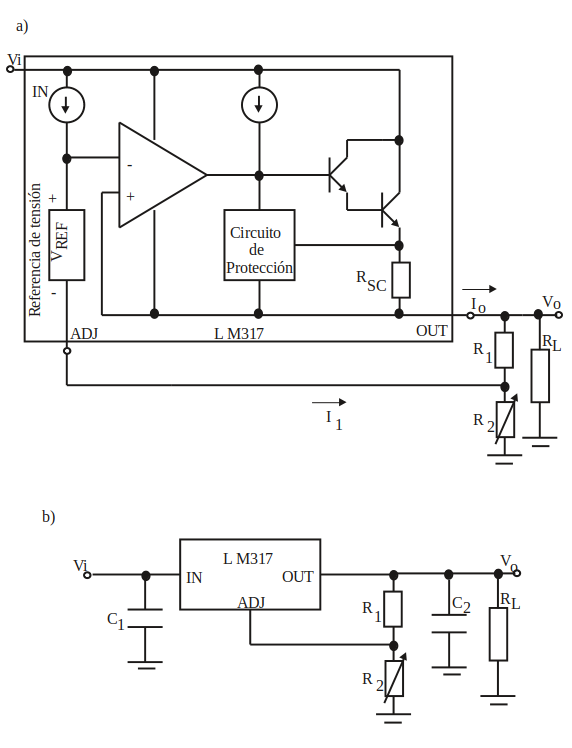
\includegraphics[width=3.5in]{figuras/fuentes20.png}\\
	\caption{Regulador de tensión con LM317: a) Diagrama en bloques del circuito integrado, b)
		implementación del regulador.}\label{fuentes20}
\end{figure}
